\documentclass[tikz,border=10pt]{standalone}
\usepackage{amsmath}

\begin{document}
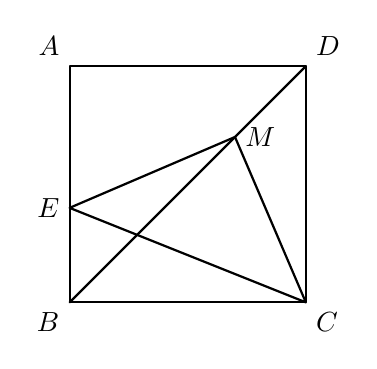
\begin{tikzpicture}[thick, >=stealth, scale=1.5, line join=round, line cap=round]
    \draw (0,2) node[above left]{$A$} -- (2,2) node[above right]{$D$} -- (2,0) node[below right]{$C$} -- (0,0) node[below left]{$B$} -- cycle;
    \draw (0,0) -- (2,2); % BD
    
    \coordinate (M) at (1.4, 1.4);
    \coordinate (E) at (0, 0.8);
    
    \draw (E) node[left]{$E$} -- (M) node[right]{$M$} -- (2,0)--(E);
    
\end{tikzpicture}
\end{document}